%\section{Cơ sở lý thuyết}
\section{CỞ SỞ LÝ THUYẾT}

\subsection{Mã hóa kênh truyền trong lĩnh vực truyền thông thông tin}

\begin{figure}[H]
	\centering
	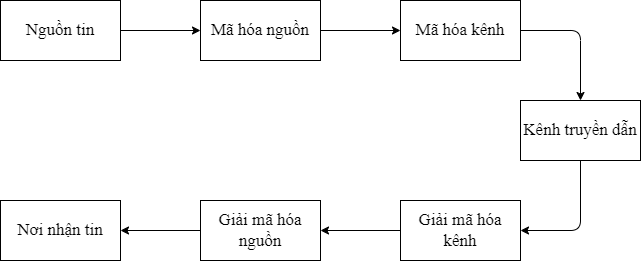
\includegraphics[width=0.6\linewidth]{sections/pic/cosolythuyet/ma-hoa-kenh.png}
	\caption{Mô hình hệ thống truyền thông số.}
	\label{f_mo-hinh-he-thong-truyen-thong-so}
\end{figure}

Mã hóa kênh truyền (Channel Coding) là một khâu quan trọng trong hệ thống truyền thông tin cùng với khối mã hóa nguồn. Mã hóa kênh là kỹ thuật thêm thông tin dư thừa (redundant information) vào tín hiệu gốc trước khi truyền để phát hiện và/hoặc sửa lỗi trong quá trình truyền qua kênh nhiễu.

Ở hình \ref{f_mo-hinh-he-thong-truyen-thong-so} thể hiện hệ thống truyền thông đơn giản trong đó,
\begin{itemize}[label=-]
	\item Nguồn tin: là nơi tạo ra thông tin cần truyền đi hay là thông tin mong muốn truyền.
	\item Mã hóa nguồn: là bộ mã hóa cho phép loại bỏ những thông tin dư thừa của chuỗi đầu vào.
	\item Mã hóa kênh: là bộ mã hóa cho phép ghép thêm các thông tin dư thừa vào chuỗi đầu vào.
	\item Kênh truyền dẫn: là các phương thức truyền thông tin có thể là không dây hoặc là hữu tuyến, vệ tinh.
\end{itemize}

Việc thêm khối mã hóa kênh vào hệ thống truyền thông số là do thường tín hiệu trong truyền thông thực tế sẽ thường xảy ra các lỗi như: Lỗi ngầu nhiên (Random Errors) do nhiễu trắng Gaussian (AWGN), Lỗi theo cụm (Burst Errors) do fading đa đường hoặc mất gói dữ liệu trong truyền thông không dây. Vì vậy, cần thêm khối mã hóa kênh vào để giúp cải thiện tỷ lệ lỗi bit (BER - Bit Error Rate) mà không cần tăng công suất truyền, còn giúp đảm bảo tính toàn vẹn của dữ liệu trong truyền thông không dây, hữu tuyến, và vệ tinh.

Có các loại mã hóa kênh phổ biến là:
\begin{itemize}[label = -]
	\item Mã khối (Block Codes): Dữ liệu được chia thành các khối có độ dài cố định, và các bit dư thừa thêm vào mỗi khối. Ví dụ: Mã Hamming, Mã Reed-Solomon.
	\item Mã chập (Convolutional Codes): Dữ liệu được mã hóa liên tục thông qua một bộ mã hóa dựa vào các thanh ghi dịch và phép toán XOR. Đặc trưng bởi các tham số: Độ dài ràng buộc (Constraint length), Tỷ lệ mã hóa (Code rate).
	\item Mã Turbo (Turbo Codes): Kết hợp nhiều bộ mã hóa và sử dụng kỹ thuật lặp (Iterative decoding) để đạt hiệu suất gần với giới hạn lý thuyết.
	\item Mã LDPC (Low-Density Parity-Check Codes): Sử dụng ma trận kiểm tra chẵn lẻ (Parity-check matrix) thưa thớt để đạt hiệu suất cao.
\end{itemize}

\subsection{Mã hóa sử dụng Mã chập (Convolutional Encoder)}

\begin{figure}[H]
	\centering
	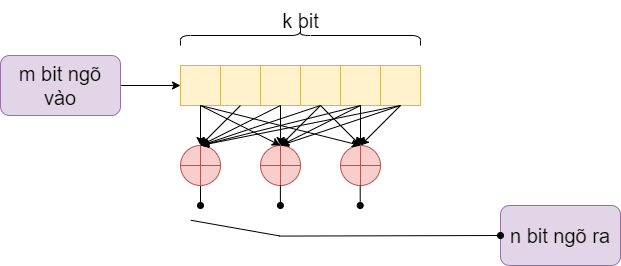
\includegraphics[width=.7\linewidth]{sections/pic/cosolythuyet/structure_convolutional_code.png}
	\caption{Cấu trúc tổng quát của một bộ mã hóa chập}
	\label{f_structure-convolutional-code}
\end{figure}

Mã chập được tạo ra bằng cách cho chuỗi thông tin truyền qua hệ thống các thanh ghi dịch tuyến tính có số trạng thái hữu hạn. Số lượng thanh ghi là \( K \), trong đó \( L = K + 1\) là \textbf{chiều dài ràng buộc} (constraint length). Bộ mã hóa chập có \( m \) bit ngõ vào và \( n \) bit ngõ ra. Tốc độ mã là \( r = m/n \), là tỉ số giữa số bit ngõ vào và số bit ngõ ra của tín hiệu. Tham số \( K \) thể hiện số lượng bit đầu vào (bao gồm bit đầu vào hiện tại và các bit đầu vào trước đó được lưu trong thanh ghi) ảnh hưởng đến đầu ra.

Một bộ mã hóa chập có cấu trúc gồm các thanh ghi dịch và các bộ cộng modulo-2. Các thanh ghi dịch lưu trữ các bit đầu vào trước đó, và các bộ cộng modulo-2 kết hợp các bit đầu vào hiện tại với các bit trong thanh ghi để tạo ra các bit đầu ra. 

Giả sử, $u$ là vector đầu vào, $x$ là vector đầu ra tương ứng được mã hóa từ vector $u$, bây giờ chúng ta mô tả cách tạo ra $x$ từ $u$. Để mô tả bộ mã hóa chúng ra cần phải kết nối vector $u$ vào thanh ghi đầu vào và $x$ vào thanh ghi đầu ra trong hình \ref{f_structure-convolutional-code}. Để có thể tính toán một cách dễ dàng, chúng ta tiến hành mô hình hóa bộ mã ở hình \ref{f_structure-convolutional-code} thành một ma trận sinh $G$ có dạng :

\[
\mathbf{G} = 
\begin{bmatrix}
	g_{1,0} & g_{1,1} & g_{1,2} & \cdots & g_{1,K-1} \\
	g_{2,0} & g_{2,1} & g_{2,2} & \cdots & g_{2,K-1} \\
	\vdots & \vdots & \vdots & \ddots & \vdots \\
	g_{n,0} & g_{n,1} & g_{n,2} & \cdots & g_{n,K-1}
\end{bmatrix}
\]

Trong đó:
\begin{itemize}[label = -]
	\item \( g_{i,j} \): Hệ số kết hợp (0 hoặc 1) cho biết bit đầu vào thứ \( j \) có tham gia vào bit đầu ra thứ \( i \) hay không.
	\item \( g_{i,j} = 1 \): Bit đầu vào thứ \( j \) được sử dụng để tính bit đầu ra thứ \( i \).
	\item \( g_{i,j} = 0 \): Bit đầu vào thứ \( j \) không được sử dụng để tính bit đầu ra thứ \( i \).
\end{itemize}

Vậy để được vector $x$ thì ta chỉ cần thực hiện phép nhân ma trận $G$ và vector $u$ lại với nhau: 
\[ x = u \cdot G \]

Để hiểu và phân tích Mã chập, có nhiều phương pháp biểu diễn khác nhau. Mỗi phương pháp biểu diễn có mục đích và ứng dụng riêng, giúp thiết kế, phân tích và triển khai mã chập một cách hiệu quả. Tuy nhiên, có các phương pháp chính sau \footnote{Để trực quan hơn, sau đây ta sẽ biểu diễn một bộ mã hóa chập đơn giản sau với $K = 3, n = 2, m = 1$.}:

\begin{figure}[H]
	\centering
	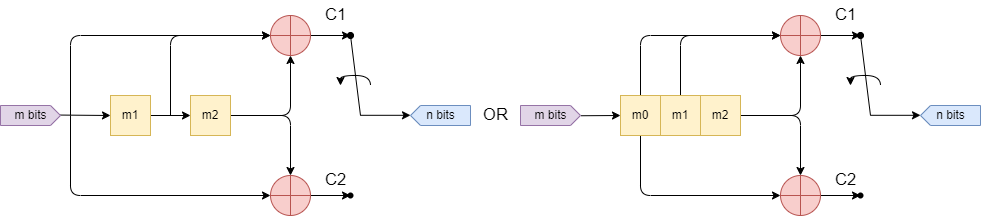
\includegraphics[width=\linewidth]{sections/pic/cosolythuyet/block_convolutional_encoder.png}
	\caption{Bộ mã hóa $(3, 1, 2)$.}
	\label{f_ex_block_conv_encoder}
\end{figure}

Trong đó, $C1 = m + m_1 + m_2$ và $C2 = m + m_2$.

\subsubsection{Ma trận sinh (Generator matrix)}

Sử dụng phương pháp biểu diễn mã chập bằng ma trận sinh, ta có thể lấy bộ mã hóa ở hình \ref{f_ex_block_conv_encoder} để thể hiện cách hoạt động của ma trận sinh. Từ hình \ref{f_ex_block_conv_encoder} ta có thể suy ra ma trận sinh $G$ là:
\[
\mathbf{G} = 
\begin{bmatrix}
	1 & 1 & 1 \\
	1 & 0 & 1 	
\end{bmatrix}
\]

Giả sử, $m_t = 1\text{, } m_{t - 1} = 0\text{, } m_{t - 2} = 1$, khi đó:
\[n = m \cdot G = \begin{bmatrix}
	m_t & m_{t - 1} & m_{t - 2}
\end{bmatrix} \cdot \begin{bmatrix}
	1 & 1 & 1 \\
	1 & 0 & 1 	
\end{bmatrix} = \begin{bmatrix}
	1 & 0 & 1
\end{bmatrix} \cdot \begin{bmatrix}
	1 & 1 & 1 \\
	1 & 0 & 1 	
\end{bmatrix} = \begin{bmatrix}
	0 & 0
\end{bmatrix}\]

\subsubsection{Sơ đồ lưới (Trellis Diagram)}

Sơ đồ trạng thái biểu diễn các trạng thái của thanh ghi và các chuyển tiếp giữa các trạng thái dựa trên bit đầu vào và bit đầu ra. Trong sơ đồ trạng thái, mỗi nút biểu diễn cho một trạng thái của thanh ghi. Các nội dung biểu diễn chuyển tiếp giữa các trạng thái, được gán nhãn bởi bit vào vầ bit đầu ra tương ứng. 

Để làm rõ hơn việc sử dụng sơ đồ trạng thái trong việc biểu diễn mã chập, ta sử dụng một bộ mã hóa chập ở hình \ref{f_ex_block_conv_encoder}. Với $K=3$ ta có tương ứng với 4 trạng thái là: \texttt{S0(00)}, \texttt{S1(01)}, \texttt{S2(10)}, \texttt{S3(11)}, và trạng thái chuyển tiếp có thể được tạo từ trạng thái này sang trạng thái khác, quá trình chuyển tiếp có thể là:

\begin{table}[H]
	\centering
	\begin{tabular}{|c|c|c|c|c|}
		\hline
		& \multicolumn{2}{c|}{Next State, if} & \multicolumn{2}{c|}{Output symbol, if} \\ \hline
		Current State & Input = 0 & Input = 1 & Input = 0 & Input = 1 \\ \hline
		S0 & S0 & S2 & 00 & 11 \\ \hline
		S1 & S0 & S2 & 11 & 00 \\ \hline
		S2 & S1 & S3 & 10 & 01 \\ \hline
		S3 & S1 & S3 & 01 & 10 \\ \hline
	\end{tabular}
	\caption{Bảng chuyển trạng thái của mã chập \( (3,1,2) \).}
	\label{t_fsm_conv_encoder}
\end{table}

Sơ đồ lưới là một mở rộng của sơ đồ trạng thái theo thời gian, biểu diễn tất cả các đường đi có thể của mã chập qua các bước thời gian. Sơ đồ lưới bao gồm các nút biểu diễn trạng thái tại mỗi bước thời gian. Các cung biểu diễn chuyển tiếp giữa các trạng thái, được gán nhãn bởi bit đầu vào và bit đầu ra.

Ở hình \ref{f_ex_block_conv_encoder}, ta có thể biểu diễn một cung chuyển tiếp đơn giản giữa hai đơn vị thời gian như sau:

\begin{figure}[H]
	\centering
	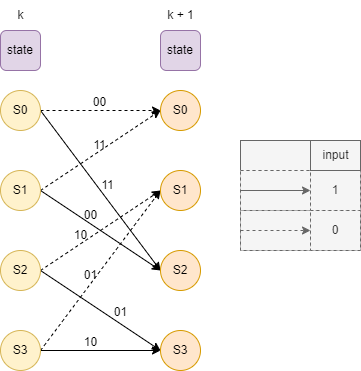
\includegraphics[width=.5\linewidth]{sections/pic/cosolythuyet/trellis-fsm-convolutional-code-coban.png}
	\caption{Sơ đồ lưới giữa hai đơn vị thời gian của bộ mã hóa $(3, 1, 2)$.}
	\label{f_trellis_unit_conv_encoder}
\end{figure}

Từ đó, ta có thể biểu diễn hoàn chỉnh cách biểu diễn bộ mã hóa chập bằng sơ đồ lưới như sau:

\begin{figure}[H]
	\centering
	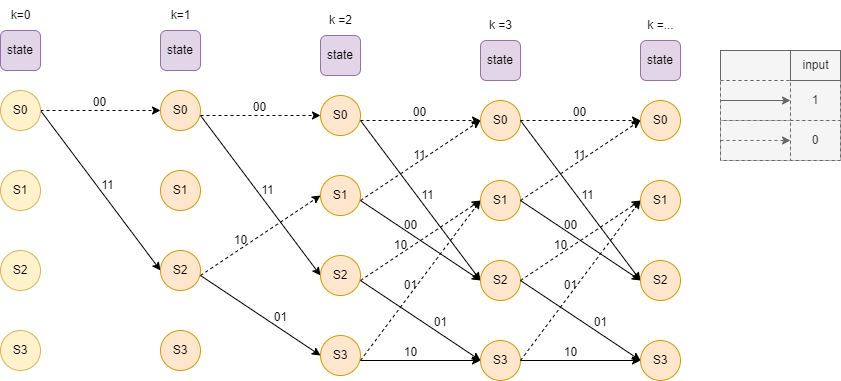
\includegraphics[width = \linewidth]{sections/pic/cosolythuyet/trellis-fsm-convolutional-code.png}
	\label{f_trellis_conv_encoder}
\end{figure}

Giả sử, chuỗi bit ngõ vào là \texttt{0101} thì ngõ ra tương ứng với chuỗi bit sau khi được mã hóa sẽ là \texttt{00 11 10 00}.

\subsection{Giải mã kênh truyền trong lĩnh vực truyền thông thông tin}

Giải mã kênh truyền là quá trình khôi phục thông tin gốc từ tín hiệu đã được mã hóa trên kênh truyền. Nó là bước ngược lại của quá trình mã hóa kênh, nhằm đưa dữ liệu về trạng thái ban đầu. Hiệu quả của giải mã kênh phụ thuộc vào nhiều yếu tố, bao gồm mô hình trạng thái và phương pháp giải mã được sử dụng. Mục tiêu chính là giảm thiểu lỗi trong quá trình truyền dữ liệu.

Ở hình \ref{f_mo-hinh-he-thong-truyen-thong-so} thể hiện hệ thống truyền thông đơn giản trong đó,

\begin{itemize}[label=-]
	\item Giải mã nguồn: khôi phục dữ liệu nguồn.
	\item Giải mã kênh: sửa lỗi do nhiễu trong quá trình truyền dẫn, đảm bảo dữ liệu nhận được gần nhất với dữ liệu gốc.
\end{itemize}

\subsection{Giải mã kênh truyền sửa dụng thuật toán Viterbi}

Thuật toán Viterbi là một giải pháp được sử dụng phổ biến để giải mã chuỗi bit được mã hóa bởi bộ mã hóa tích chập. Chi tiết của một bộ giải mã riêng phụ thuộc vào một bộ mã hóa tích chập tương ứng. Thuật toán Viterbi không phải là một thuật toán đơn lẻ có thể dùng để giải mã những chuỗi bit mà được mã hóa bởi bất cứ một bộ mã hóa chập nào.

Thuật toán Viterbi được khởi xướng bởi Andrew Viterbi vào năm 1967 như là một thuật toán giải mã cho mã chập qua các tuyến thông tin có nhiễu. Nó được sử dụng trong cả hai hệ thống CDMA và GSM, các modem số, vệ tinh, thông tin vũ trụ, và các hệ thống mạng cục bộ không dây. Hiện nay còn được sử dụng phổ biến trong kỹ thuật nhận dạng giọng nói, nhận dạng từ mã, ngôn ngữ học máy tính.

Thuật toán Giải mã Vitervi là một trong hai loại thuật toán giải mã được sử dụng với bộ mã hóa chập - là một loại giải mã tuần tự. Ưu điểm của giải mã tuần tự so với Viterbi là nó có thể hoạt động tốt với các mã chập có chiều dài ràng buộc lớn, nhưng nó lại có thời gian giải mã biến đổi.

Còn ưu điểm cảu thuật toán Giải mã Viterbi là nó có thời gian mã ổn định. Điều đó rất tốt cho việc thực thi bộ giải mã bằng phần cứng. Nhưng mà yêu cầu về sự tính toán của nó tăng theo hàm mũ như là một hàm của chiều dài rằng buộc. Vì vậy trong thực tế, người ta thường giới hạn chiều dài ràng buộc của nó là 9 ($k \leq 9$).

Thuật toán Viterbi là một giải pháp giải mã tối ưu cho các chuỗi bit được mã hóa bởi bộ mã hóa tích chập (convolutional encoder). Đây là thuật toán quyết định cứng (hard-decision) sử dụng nguyên lý quy hoạch động để tìm chuỗi trạng thái có xác suất cao nhất trong lưới trạng thái (trellis diagram).

\subsubsection*{Đặc điểm chính}
\begin{itemize}[label=-]
	\item \textbf{Tính tương thích}: Mỗi bộ giải mã Viterbi phải được thiết kế tương ứng với một bộ mã hóa tích chập cụ thể.
	
	\item \textbf{So sánh với giải mã tuần tự}:
	\begin{itemize}[label=+]
		\item Ưu điểm: Hiệu suất giải mã ổn định, độ phức tạp tính toán thấp
		\item Nhược điểm: Khó áp dụng cho mã có độ dài ràng buộc (constraint length) lớn
	\end{itemize}
	
	\item \textbf{Ứng dụng}:
	\begin{itemize}[label=+]
		\item Hệ thống thông tin di động (GSM, CDMA)
		\item Truyền dẫn vệ tinh
		\item Nhận dạng tiếng nói
	\end{itemize}
\end{itemize}

\subsubsection*{Nguyên lý hoạt động}
Thuật toán thực hiện các bước chính:
\begin{enumerate}
	\item Khởi tạo metric cho các trạng thái
	\item Tính toán độ tương đồng (branch metric)
	\item Cập nhật path metric
	\item Truy vết ngược (traceback) để tìm chuỗi giải mã tối ưu
\end{enumerate}

Phương trình cập nhật metric:
\[
\gamma_t(s',s) = \gamma_{t-1}(s') + \sum_{i=1}^n (r_i^{(t)} - c_i^{(t)})^2
\]
trong đó:
\begin{itemize}
	\item $s', s$: các trạng thái liên tiếp
	\item $r_i^{(t)}$: bit nhận được tại thời điểm t
	\item $c_i^{(t)}$: bit mã hóa tương ứng
\end{itemize}